% !TeX root = proyecto.tex

%=========================================================
\chapter{Modelo dinámico}	
\label{cap:modDinamico}

\cdtInstrucciones{Presente la solución indicando el si esta se compone de varios sistemas, los subsistemas del sistema y si aplica, los módulos de los subsistemas.}

	Este capítulo describe en modelo dinámico del sistema. en el se detallan todos los escenarios de ejecución del sistema. La figura~\ref{fig:casosDeUso} muestra el diagrama general del sistema y sus subsistemas, y la figura~\ref{fig:casosDeUsoDetalle} muestra todos los casos de uso del sistema. En este documento solo detallamos los casos de uso del subsistema de gestión de cursos.
	
\begin{figure}[htbp]
	\begin{center}
		\fbox{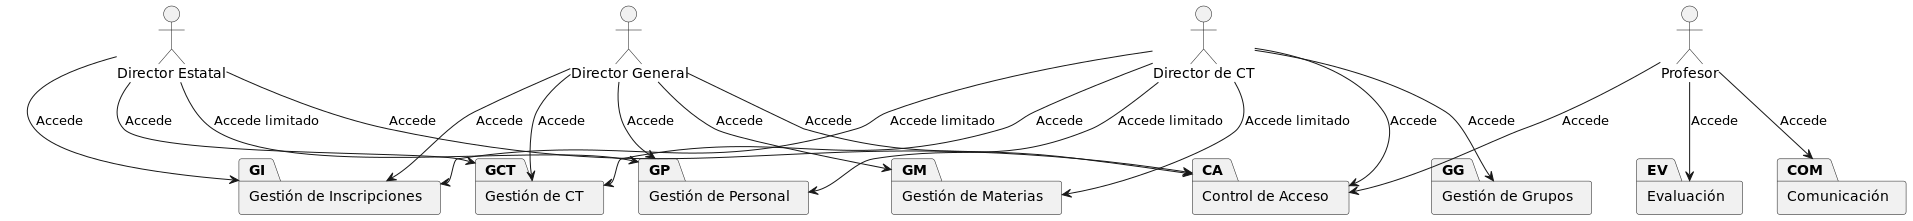
\includegraphics[width=.8\textwidth]{images/casosDeUso}}
		\caption{Diagrama de casos de uso del sistema.}
		\label{fig:casosDeUso}
	\end{center}
\end{figure}

\begin{figure}[htbp]
	\begin{center}
		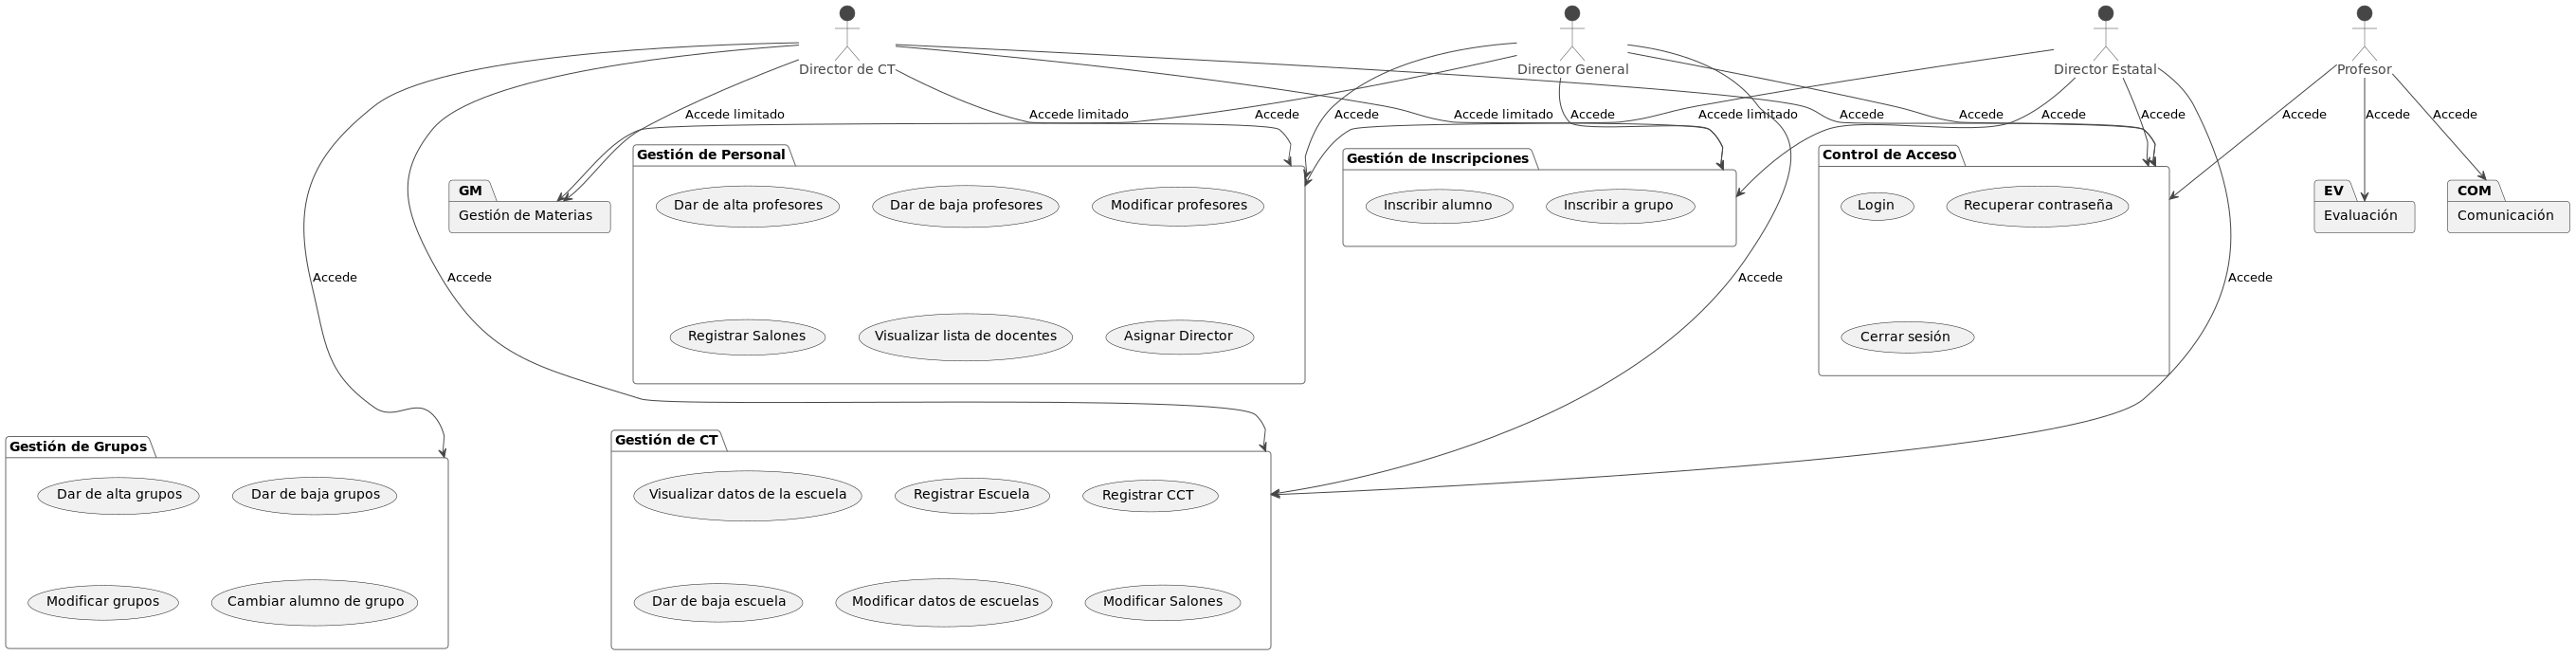
\includegraphics[ width=1.1\textwidth]{images/casosDeUsoDetalle}
		\caption{Diagrama detallado del sistema.}
		\label{fig:casosDeUsoDetalle}
	\end{center}
\end{figure}

%---------------------------------------------------------
\section{Descripción de casos de uso}



A continuación se detallan los casos de uso.

%---------------------------------------------------------
% CASOS DE USO

%%!TEX root = ../proyecto.tex

% Plantilla para caso de uso sencillo con ejemplos de comandos e intrucciones.
%-------------------------------------- COMIENZA descripción del caso de uso.

%\begin{UseCase}[archivo de imágen]{UCX}{Nombre del Caso de uso}{
%--------------------------------------
\begin{UseCase}{CUX}{Escriba el nombre del caso de uso}{
	% La descripción debe describir el evento de inicio del caso de uso, Breve descripción de la trayectoria y estado final del caso de uso.
}
	\UCitem{Versión}{\color{Gray}
		0.1	% Ponga un número de versión, 
	}\UCitem{Autor}{\color{Gray}
		Nombre del analista. % Analista responsable de especificar el CU
	}\UCitem{Supervisa}{\color{Gray}
		Nombre del analista revisor. % Analista responsable de verificar que está correcto.
	% TODO: Dar de alta al actor Usuario
	}\UCitem{Actor}{
		\hyperlink{IdDelActor}{Nombre del actor} % No olvide dar de alta el actor.
	}\UCitem{Propósito}{\begin{Titemize}%Indique los fines, objetivos, propósitos o valores agregados del Caso de uso.
		\Titem Propósito del caso de uso.
		\Titem ...
	\end{Titemize}
	}\UCitem{Entradas}{\begin{Titemize}
		% TODO: Dar de alta las entidades que se listan.
		\Titem \hyperlink{Entidad.Atributo}{Nombre del dato de entrada}. % El identificador no acepta acentos, espacios ni eñes.
		\Titem \hyperlink{Entidad.Atributo}{Nombre del dato de entrada}. % Liste todos los datos de entrada
		\end{Titemize}
	}\UCitem{Origen}{\begin{Titemize}
		\Titem Se introducen desde el teclado. % Indique por que medio se introducen los datos, 
		\Titem otros.          % Si es ḿas de uno indique que datos corresponden en cada medio de entrada.
	\end{Titemize}
	}\UCitem{Salidas}{\begin{Titemize}
		% TODO: Dar de alta las entidades que se listan.
		\Titem \hyperlink{Entidad.Atributo}{Nombre del dato de entrada}.
		\Titem Mensajes de error. % Indique por que medio se introducen los datos, 
		\Titem Datos que aparecen en pantalla.          % Si es ḿas de uno indique que datos corresponden en cada medio de entrada.
		\Titem Datos que aparecen en listas desplegables o tablas, etc.
		\Titem Datos que se imprimen o que se envía a otros sistemas.
	\end{Titemize}
	}\UCitem{Destino}{\begin{Titemize}
		\Titem Se muestra en la pantalla \IUref{IUX}{Nombre pantalla}.. % Indique por que medio se muestran los datos, 
		\Titem otros.          % Si es ḿas de uno indique que datos corresponden en cada medio de entrada.
	\end{Titemize}
	}\UCitem{Precondiciones}{\begin{Titemize}
		% Incluya Precondiciones lógicas, de negocio e incluso las que debe atender el usuario. 
		% Muchas precondiciones provienen de reglas de negocios, otras estarán asociadas a manejo de errores
		% Otras están relacionadas con casos de uso que deben ejecutarse previamente, como registrar un producto.
		\Titem Escriba la precondición.
	\end{Titemize}
	}\UCitem{Postcondiciones}{\begin{Titemize}
		% Indique todas las postcondiciones
		% por ejemplo, Cambios en el sistema
		% Cambios en la BD una vez terminado el CU
		% Efectos colaterales
		% Condiciones de término.
		\Titem Escriba todas las postcondiciones.
	\end{Titemize}
	}\UCitem{Errores}{\begin{Titemize}
		% Escriba todos los errores que puedan ocurrir en el sistema, para cada error recuerde:
		% Punerle un identificador
		% Describir la condición o escenario que detona el error
		% Describa la forma en que debe reaccionar el sitema: si la reaccion corresponde a varios pasos use mejor una trayectoria alternativa.
		% Relacione el error con la trayectoria principal.
		\Titem {\bf \hypertarget{CUX.E1}{E1}}: Condición que detona el error, reacción del sistema y regresa al paso \ref{UC1.etiqueta}.
		\Titem {\bf \hypertarget{CUX.E2}{E2}}: Condición que detona el error, reacción del sistema y termina el Caso de uso..
	\end{Titemize}
	}\UCitem{Tipo}{
		% Especifique el tipo de caso de us, puede ser: "Caso de uso primario" o 
		% "Viene de \\hyperref{CUY}{CUY nombre del CU}" cuando se desprende desde otro caso de uso mediante un extends.
		Caso de uso primario
	}\UCitem{Observaciones}{
		% Indique las observaciones al caso de uso, las cuales pueden ser:
		% - Ninguna
		% - Dudas sobre el procedimiento o la especificación.
		% - Issues detectados
		% - Suposiciones realizadas.
		% - Cualquier otra especificacion que considere pertinente que no pudo colocarse en los demás atributos del Caso de uso
		% - Aclaraciones.
		% - Notas para el usuario o desarrollador.
		% - Pendientes (TODO's) en caso de no usar los comentarios.
	}
\end{UseCase}

%--------------------------------------
\begin{UCtrayectoria}
	% Cada paso debe inicair con un Verbo en infinitivo, siempre especificando el objetivo del paso mas la accion en concreto.
	% \UCpaso[\UCactor] se refiere al actor y \UCpaso se refiere al sistema.
	% A continuación viene ejemplos de pasos:
	% En el siguiente paso: "Ingresa al sistema" es el objetivo del paso y "escribiendo la URL de la aplicación" es la acción en concreto.
	\UCpaso[\UCactor o \UCsist] VERBO EN INFINITIVO + (Acción del usuario) + (Acción dentro del sistema)
	\UCpaso[\UCactor] Ingresa al sistema escribiendo la URL de la aplicación.
	% En el siguinte paso se referencia una Interfaz:
	\UCpaso Solicita al usuario que se identifique mediante la pantalla \IUref{IU1}{Inicio de sesión}
	% En el siguiente paso está etiquetado para ser referenciado por un error o trayectoria alternativa:
	\UCpaso[\UCactor] \label{UCX.introduceDatos} Se identifica introduciendo su nombre de usuario y contraseña.
	% En el siguiente paso se usa el comando \IUbutton 
	\UCpaso[\UCactor] Solicita el ingreso al sistema presiona el botón \IUbutton{Ingresar}.
	% En el siguiente paso se referencía un error.
	\UCpaso Busca los datos del usuario identificado por el nombre de usuario introducido \ErrorRef{CUX}{E1}{No hay usuario}
	% En el siguiente paso se señala una trayectoria alternativa
	\UCpaso Verifica que el usuario especificado no esté inactivo \ErrorRef{CUX}{E2}{Usuario inactivo} \Trayref{CUX}{A}.
	% En el siguiente paso se referencían dos errores y una trayectoria alternativa.
	\UCpaso Verifica que la contraseña ingresada coincida con la almacenada \ErrorRef{CUX}{E3}{La contraseña no coincide}\Trayref{CUX}{B}.
	% En el siguiente paso se señala la incusión de otro CU
	\UCpaso[] Se ejecutan los pasos del caso de uso \UCref{CUY}{Nombre del caso de uso}.
	% En el siguiente paso se señala un mensaje.
	\UCpaso Muestra la pantalla \IUref{IU2}{Principal} con el mensaje \MSGref{MSG-001}{Bienvenida al usuario}.
\end{UCtrayectoria}


%--------------------------------------
% Las trayectorias alternativas se identifican con Letras: A, B, C, etc.
\begin{UCtrayectoriaA}{CUX}{LETRA}{Condición que hace que se ejecute esta trayectoria}
	\UCpaso Especifique los pasos  de la trayectoria.
	% Se puede desprender otra trayectria alternativa si es necesario.
	% Finalice la trayectoria indicando si la ejecución se integra a la trayectoria anterior o si termina la ejecución del CU.
	% Verifique que la redacción de la trayectoria deje en claro si el objetivo del CU se alcanzó o no.
	\UCpaso[] El Caso de Uso continúa en el paso \ref{UCX.introduceDatos}.
\end{UCtrayectoriaA}


%--------------------------------------
% Puntos de extensión

% Comente la siguiente sección en caso de que no hayan puntos de extensión o relaciones de tipo extends.
\subsection{Puntos de extensión}
\UCExtenssionPoint{
	% Cuando se dá la extensión del Caso de uso:
	El usuario no recuerda cual es su contraseña o sospecha que su usuario está bloqueado.
}{
	% Durante la región (en que pasos se puede dar la extensión):
	Del paso \ref{CUX.etiqueta} al paso \ref{CUX.etiqueta}.
}{
	% Casos de uso a los que extiende:
	\UCref{CUZ}{Nombre del caso de uso}.
}
		
		
		
%-------------------------------------- TERMINA descripción del caso de uso.
%!TEX root = ../proyecto.tex

% Plantilla para caso de uso sencillo con ejemplos de comandos e intrucciones.
%-------------------------------------- COMIENZA descripción del caso de uso.

%\begin{UseCase}[archivo de imágen]{UCX}{Nombre del Caso de uso}{
%--------------------------------------
\begin{UseCase}{CU-001}{Inicio de sesión (login) }{
	% La descripción debe describir el evento de inicio del caso de uso, Breve descripción de la trayectoria y estado final del caso de uso.
 Cuando un usuario desee ingresar al sistema deberá proporcionarle sus datos de acceso y de ser correctos este le permitirá iniciar sesión.
}
	\UCitem{Versión}{\color{Gray}
		0.1	% Ponga un número de versión, 
	}\UCitem{Autor}{\color{Gray}
		Agustín Flores López. % Analista responsable de especificar el CU
	}\UCitem{Supervisa}{\color{Gray}
		Juan Ángel Serrano Carreño . % Analista responsable de verificar que está correcto.
	% TODO: Dar de alta al actor Usuario
	}\UCitem{Actor}{
		\hyperlink{Usuarios}{Usuarios} % No olvide dar de alta el actor.
	}\UCitem{Propósito}{\begin{Titemize}%Indique los fines, objetivos, propósitos o valores agregados del Caso de uso.
		\Titem Controlar el acceso al sistema.
		\Titem Restringir el uso de las funciones más sensibles solo a los perfiles adecuados.
        \Titem Permitir la trazabilidad de las operaciones en el sistema.
	\end{Titemize}
	}\UCitem{Entradas}{\begin{Titemize}
		% TODO: Dar de alta las entidades que se listan.
		\Titem \hyperlink{Usuario.ID}{Identificador} en el PRONIM. % El identificador no acepta acentos, espacios ni eñes.
		\Titem \hyperlink{Usuario.Contrasenia}{Contraseña}. % Liste todos los datos de entrada
		\end{Titemize}
	}\UCitem{Origen}{\begin{Titemize}
		\Titem Se introducen desde el teclado. % Indique por que medio se introducen los datos,           % Si es ḿas de uno indique que datos corresponden en cada medio de entrada.
	\end{Titemize}
	}\UCitem{Salidas}{\begin{Titemize}
		% TODO: Dar de alta las entidades que se listan.
		\Titem \hyperlink{Usuario.nombre}{Nombre} del \hyperlink{Usuario}{Usuario}.
            \Titem \hyperlink{Usuario.primerApellido}{Primer apellido} del \hyperlink{Usuario}{Usuario}.
		\Titem Mensajes de error. % Indique por que medio se introducen los datos, 
		         % Si es ḿas de uno indique que datos corresponden en cada medio de entrada.
		
	\end{Titemize}
	}\UCitem{Destino}{\begin{Titemize}
		\Titem Se muestra en la pantalla \IUref{IU001}{Inicio de sesión}.. % Indique por que medio se muestran los datos, 
          % Si es ḿas de uno indique que datos corresponden en cada medio de entrada.
	\end{Titemize}
	}\UCitem{Precondiciones}{\begin{Titemize}
		% Incluya Precondiciones lógicas, de negocio e incluso las que debe atender el usuario. 
		% Muchas precondiciones provienen de reglas de negocios, otras estarán asociadas a manejo de errores
		% Otras están relacionadas con casos de uso que deben ejecutarse previamente, como registrar un producto.
		\Titem El usuario debe estar registrado en el sistema.
	\end{Titemize}
	}\UCitem{Postcondiciones}{\begin{Titemize}
		% Indique todas las postcondiciones
		% por ejemplo, Cambios en el sistema
		% Cambios en la BD una vez terminado el CU
		% Efectos colaterales
		% Condiciones de término.
		\Titem El usuario inicia sesión en el sistema.
            \Titem El usuario puede acceder a las funciones de su rol.
	\end{Titemize}
	}\UCitem{Errores}{\begin{Titemize}
		% Escriba todos los errores que puedan ocurrir en el sistema, para cada error recuerde:
		% Punerle un identificador
		% Describir la condición o escenario que detona el error
		% Describa la forma en que debe reaccionar el sitema: si la reaccion corresponde a varios pasos use mejor una trayectoria alternativa.
		% Relacione el error con la trayectoria principal.
		\Titem {\bf \hypertarget{CU001.E1}{E1}}: Si el usuario olvida ingresar alguno de los campos obligatorios, el sistema mostrara el \MSGref{MSG-005}{Faltan rellenar campos obligatorios}. y regresa al paso \ref{UC1.Datos}.
		\Titem {\bf \hypertarget{CU001.E2}{E2}}: Si la contraseña es incorrecta, el sistema mostrara el \MSGref{MSG-004}{Error al iniciar sesión}  y regresa al paso \ref{UC1.Datos}.
  \Titem {\bf \hypertarget{CU001.E3}{E3}}: Si la cuenta esta inactiva, el sistema mostrara el \MSGref{MSG-003}{Cuenta inactiva}  y regresa al paso \ref{UC1.Datos}.
  \Titem {\bf \hypertarget{CU001.E4}{E4}}: Si la cuenta no existe, el sistema mostrara el \MSGref{MSG-002}{Usuario no registrado}  y regresa al paso \ref{UC1.Datos}.
	\end{Titemize}
	}\UCitem{Tipo}{
		% Especifique el tipo de caso de us, puede ser: "Caso de uso primario" o 
		% "Viene de \\hyperref{CUY}{CUY nombre del CU}" cuando se desprende desde otro caso de uso mediante un extends.
		Caso de uso primario
	}\UCitem{Observaciones}{
		% Indique las observaciones al caso de uso, las cuales pueden ser:
		% - Ninguna
		% - Dudas sobre el procedimiento o la especificación.
		% - Issues detectados
		% - Suposiciones realizadas.
		% - Cualquier otra especificacion que considere pertinente que no pudo colocarse en los demás atributos del Caso de uso
		% - Aclaraciones.
		% - Notas para el usuario o desarrollador.
		% - Pendientes (TODO's) en caso de no usar los comentarios.
	}
\end{UseCase}

%--------------------------------------
\begin{UCtrayectoria}
	% Cada paso debe inicair con un Verbo en infinitivo, siempre especificando el objetivo del paso mas la accion en concreto.
	% \UCpaso[\UCactor] se refiere al actor y \UCpaso se refiere al sistema.
	% A continuación viene ejemplos de pasos:
	% En el siguiente paso: "Ingresa al sistema" es el objetivo del paso y "escribiendo la URL de la aplicación" es la acción en concreto.
	
	\UCpaso[\UCactor] Ingresa al sistema escribiendo la URL de la aplicación.
	% En el siguinte paso se referencia una Interfaz:
	\UCpaso Solicita al usuario que se identifique mediante la pantalla \IUref{IU1}{Inicio de sesión}
	% En el siguiente paso está etiquetado para ser referenciado por un error o trayectoria alternativa:
	\UCpaso[\UCactor] \label{UC1.Datos} Se identifica introduciendo su Identificador de Pronim y contraseña.
	% En el siguiente paso se usa el comando \IUbutton 
	\UCpaso[\UCactor] Solicita el ingreso al sistema presiona el botón \IUbutton{Ingresar}.
	% En el siguiente paso se referencía un error.
    \UCpaso Verifica que todos los campos obligatorios esten llenos \ErrorRef{CU001}{E1}{Campos faltantes}.
	\UCpaso Busca los datos del usuario identificado por el Identificador introducido \ErrorRef{CU001}{E4}{Usuario no registrado}
	% En el siguiente paso se señala una trayectoria alternativa
	\UCpaso Verifica que el usuario especificado no esté inactivo \ErrorRef{CU001}{E3}{Usuario inactivo}.
	% En el siguiente paso se referencían dos errores y una trayectoria alternativa.
	\UCpaso Verifica que la contraseña ingresada coincida con la almacenada \ErrorRef{CU001}{E2}{La contraseña no coincide}.\label{UC1.Contrasenia}
	% En el siguiente paso se señala la incusión de otro CU
	\UCpaso Verifica su rol dentro del sistema y le otorga los permisos correspondientes
	% En el siguiente paso se señala un mensaje.
	\UCpaso Muestra la pantalla \IUref{IU2}{Principal} con el mensaje \MSGref{MSG-001}{Bienvenida al usuario}.
\end{UCtrayectoria}


%--------------------------------------
% Las trayectorias alternativas se identifican con Letras: A, B, C, etc.



%--------------------------------------
% Puntos de extensión

% Comente la siguiente sección en caso de que no hayan puntos de extensión o relaciones de tipo extends.
\subsection{Puntos de extensión}
\UCExtenssionPoint{
	% Cuando se dá la extensión del Caso de uso:
	El usuario no recuerda cual es su contraseña .
}{
	% Durante la región (en que pasos se puede dar la extensión):
	Del paso \ref{UC1.Datos} al paso \ref{UC1.Contrasenia}.
}{
	% Casos de uso a los que extiende:
	\UCref{CUX}{Nombre del caso de uso}.
}
		
		
		
%-------------------------------------- TERMINA descripción del caso de uso.
%!TEX root = ../proyecto.tex

% Plantilla para caso de uso sencillo con ejemplos de comandos e intrucciones.
%-------------------------------------- COMIENZA descripción del caso de uso.

%\begin{UseCase}[archivo de imágen]{UCX}{Nombre del Caso de uso}{
%--------------------------------------
\begin{UseCase}{CU-002}{Visualizar lista de escuelas (Suponiendo filtro y sesión necesaria)}{
	% La descripción debe describir el evento de inicio del caso de uso, Breve descripción de la trayectoria y estado final del caso de uso.
 Dado un inicio de sesión exitoso, el usuario puede dar clic en consultar escuelas,lo cual lo llevara a la IU002 que cambiara su contenido dependiendo del filtro aplicado por el usuario (Nombre de escuela,Nivel educativo,Estado,Lenguas)
}
	\UCitem{Versión}{\color{Gray}
		0.1	% Ponga un número de versión, 
	}\UCitem{Autor}{\color{Gray}
		Juan Ángel Serrano Carreño. % Analista responsable de especificar el CU
	}\UCitem{Supervisa}{\color{Gray}
		Agustín Flores López. % Analista responsable de verificar que está correcto.
	% TODO: Dar de alta al actor Usuario
	}\UCitem{Actor}{
		\hyperlink{Usuarios}{Usuarios} % No olvide dar de alta el actor.
	}\UCitem{Propósito}{\begin{Titemize}%Indique los fines, objetivos, propósitos o valores agregados del Caso de uso.
		\Titem Consultar la disponibilidad del PRONIM en una zona especifica
        \Titem Filtrar las escuelas que cumplan alguna de las siguientes características (Nombre de escuela,Nivel educativo,Estado,Lenguas)
	\end{Titemize}
	}\UCitem{Entradas}{\begin{Titemize}
		% TODO: Dar de alta las entidades que se listan.
        \Titem Nombre de la escuela (opcional)
		\Titem Nombre del estado (opcional)
        \Titem Escolaridad (opcional)
        \Titem Lenguas que permite (opcional)
		\end{Titemize}
	}\UCitem{Origen}{\begin{Titemize}
		\Titem Se introducen desde el teclado y el mouse para los selectores. % Indique por que medio se introducen los datos,           % Si es ḿas de uno indique que datos corresponden en cada medio de entrada.
	\end{Titemize}
	}\UCitem{Salidas}{\begin{Titemize}
		% TODO: Dar de alta las entidades que se listan.
		\Titem Listado de escuelas que cumplan con los filtros y que al dar clic los lleve al perfil de la escuela
        \Titem Mensaje de información 
	\end{Titemize}
	}\UCitem{Destino}{\begin{Titemize}
		\Titem Se muestra en la pantalla \IUref{IU002}{Listas de escuelas}.. % Indique por que medio se muestran los datos, 
          % Si es ḿas de uno indique que datos corresponden en cada medio de entrada.
	\end{Titemize}

% AQUI ME QUEDE
 
	}\UCitem{Precondiciones}{\begin{Titemize}
		% Incluya Precondiciones lógicas, de negocio e incluso las que debe atender el usuario. 
		% Muchas precondiciones provienen de reglas de negocios, otras estarán asociadas a manejo de errores
		% Otras están relacionadas con casos de uso que deben ejecutarse previamente, como registrar un producto.
		\Titem Debe haber un login exitoso en la plataforma.
	\end{Titemize}
	}\UCitem{Postcondiciones}{\begin{Titemize}
		% Indique todas las postcondiciones
		% por ejemplo, Cambios en el sistema
		% Cambios en la BD una vez terminado el CU
		% Efectos colaterales
		% Condiciones de término.
		\Titem Modificación de la lista a mostrar.
	\end{Titemize}
	}\UCitem{Errores}{\begin{Titemize}
		% Escriba todos los errores que puedan ocurrir en el sistema, para cada error recuerde:
		% Punerle un identificador
		% Describir la condición o escenario que detona el error
		% Describa la forma en que debe reaccionar el sitema: si la reaccion corresponde a varios pasos use mejor una trayectoria alternativa.
		% Relacione el error con la trayectoria principal.
		\Titem {\bf \hypertarget{CU002.E1}{E1}}: Dado una selección de filtros, no se encontró ningún elemento que los cumpla de forma que mostrara \MSGref{MSG-006}{No se encontró información}.
	\end{Titemize}
	}\UCitem{Tipo}{
		% Especifique el tipo de caso de us, puede ser: "Caso de uso primario" o 
		% "Viene de \\hyperref{CUY}{CUY nombre del CU}" cuando se desprende desde otro caso de uso mediante un extends.
		Caso de uso primario
	}\UCitem{Observaciones}{
		% Indique las observaciones al caso de uso, las cuales pueden ser:
		% - Ninguna
		% - Dudas sobre el procedimiento o la especificación.
		% - Issues detectados
		% - Suposiciones realizadas.
		% - Cualquier otra especificacion que considere pertinente que no pudo colocarse en los demás atributos del Caso de uso
		% - Aclaraciones.
		% - Notas para el usuario o desarrollador.
		% - Pendientes (TODO's) en caso de no usar los comentarios.
        Tiene que incluir los filtros y que se pueda ver unicamente si esta iniciado en sesión 
	}
\end{UseCase}

%--------------------------------------
\begin{UCtrayectoria}
	% Cada paso debe inicair con un Verbo en infinitivo, siempre especificando el objetivo del paso mas la accion en concreto.
	% \UCpaso[\UCactor] se refiere al actor y \UCpaso se refiere al sistema.
	% A continuación viene ejemplos de pasos:
	% En el siguiente paso: "Ingresa al sistema" es el objetivo del paso y "escribiendo la URL de la aplicación" es la acción en concreto.
	\UCpaso[\UCactor] Ingresa a la búsqueda de escuela dando clic en la opción buscar escuela de la interfaz principal (pendiente)
	% En el siguinte paso se referencia una Interfaz:
	\UCpaso Solicita al usuario que se identifique mediante la pantalla \IUref{IU2}{Listar escuelas}
	% En el siguiente paso está etiquetado para ser referenciado por un error o trayectoria alternativa:
	\UCpaso[\UCactor] \label{UCX.introduceDatos} Se identifica introduciendo su nombre de usuario y contraseña.
	% En el siguiente paso se usa el comando \IUbutton 
	\UCpaso[\UCactor] Solicita el ingreso al sistema presiona el botón \IUbutton{Ingresar}.
	% En el siguiente paso se referencía un error.
	\UCpaso Busca los datos del usuario identificado por el nombre de usuario introducido \ErrorRef{CUX}{E1}{No hay usuario}
	% En el siguiente paso se señala una trayectoria alternativa
	\UCpaso Verifica que el usuario especificado no esté inactivo \ErrorRef{CUX}{E2}{Usuario inactivo} \Trayref{CUX}{A}.
	% En el siguiente paso se referencían dos errores y una trayectoria alternativa.
	\UCpaso Verifica que la contraseña ingresada coincida con la almacenada \ErrorRef{CUX}{E3}{La contraseña no coincide}\Trayref{CUX}{B}.
	% En el siguiente paso se señala la incusión de otro CU
	\UCpaso[] Se ejecutan los pasos del caso de uso \UCref{CUY}{Nombre del caso de uso}.
	% En el siguiente paso se señala un mensaje.
	\UCpaso Muestra la pantalla \IUref{IU2}{Principal} con el mensaje \MSGref{MSG-001}{Bienvenida al usuario}.
\end{UCtrayectoria}


%--------------------------------------
% Las trayectorias alternativas se identifican con Letras: A, B, C, etc.
\begin{UCtrayectoriaA}{CUX}{LETRA}{Condición que hace que se ejecute esta trayectoria}
	\UCpaso Especifique los pasos  de la trayectoria.
	% Se puede desprender otra trayectria alternativa si es necesario.
	% Finalice la trayectoria indicando si la ejecución se integra a la trayectoria anterior o si termina la ejecución del CU.
	% Verifique que la redacción de la trayectoria deje en claro si el objetivo del CU se alcanzó o no.
	\UCpaso[] El Caso de Uso continúa en el paso \ref{UCX.introduceDatos}.
\end{UCtrayectoriaA}


%--------------------------------------
% Puntos de extensión

% Comente la siguiente sección en caso de que no hayan puntos de extensión o relaciones de tipo extends.
\subsection{Puntos de extensión}
\UCExtenssionPoint{
	% Cuando se dá la extensión del Caso de uso:
	El usuario no recuerda cual es su contraseña o sospecha que su usuario está bloqueado.
}{
	% Durante la región (en que pasos se puede dar la extensión):
	Del paso %\ref{CUX.etiqueta} al paso \ref{CUX.etiqueta}.
}{
	% Casos de uso a los que extiende:
	\UCref{CUZ}{Nombre del caso de uso}.
}
		
		
		
%-------------------------------------- TERMINA descripción del caso de uso.
%!TEX root = ../proyecto.tex

% Plantilla para caso de uso sencillo con ejemplos de comandos e intrucciones.
%-------------------------------------- COMIENZA descripción del caso de uso.

%\begin{UseCase}[archivo de imágen]{UCX}{Nombre del Caso de uso}{
%--------------------------------------
\begin{UseCase}{CU-004}{Visualizar datos de la escuela}{
	% La descripción debe describir el evento de inicio del caso de uso, Breve descripción de la trayectoria y estado final del caso de uso.
 Cuando un usuario desee ingresar al sistema debera proporcionarle sus datos de acceso y de ser correctos este le permitira iniciar sesión.
}
	\UCitem{Versión}{\color{Gray}
		0.1	% Ponga un número de versión, 
	}\UCitem{Autor}{\color{Gray}
		Agustin Flores Lopez. % Analista responsable de especificar el CU
	}\UCitem{Supervisa}{\color{Gray}
		Juan Angel Serrano Carreño . % Analista responsable de verificar que está correcto.
	% TODO: Dar de alta al actor Usuario
	}\UCitem{Actor}{
		\hyperlink{Usuarios}{Usuarios} % No olvide dar de alta el actor.
	}\UCitem{Propósito}{\begin{Titemize}%Indique los fines, objetivos, propósitos o valores agregados del Caso de uso.
		\Titem Controlar el acceso al sistema.
		\Titem Restringir el uso de las funciones más sensibles solo a los perfiles adecuados.
        \Titem Permitir la trazabilidad de las operaciones en el sistema.
	\end{Titemize}
	}\UCitem{Entradas}{\begin{Titemize}
		% TODO: Dar de alta las entidades que se listan.
		\Titem \hyperlink{Usuario.ID}{Identificador} en el PRONIM. % El identificador no acepta acentos, espacios ni eñes.
		\Titem \hyperlink{Usuario.Contrasenia}{Contraseña}. % Liste todos los datos de entrada
		\end{Titemize}
	}\UCitem{Origen}{\begin{Titemize}
		\Titem Se introducen desde el teclado. % Indique por que medio se introducen los datos,           % Si es ḿas de uno indique que datos corresponden en cada medio de entrada.
	\end{Titemize}
	}\UCitem{Salidas}{\begin{Titemize}
		% TODO: Dar de alta las entidades que se listan.
		\Titem \hyperlink{Usuario.nombre}{Nombre} del \hyperlink{Usuario}{Usuario}.
            \Titem \hyperlink{Usuario.primerApellido}{Primer apellido} del \hyperlink{Usuario}{Usuario}.
		\Titem Mensajes de error. % Indique por que medio se introducen los datos, 
		         % Si es ḿas de uno indique que datos corresponden en cada medio de entrada.
		
	\end{Titemize}
	}\UCitem{Destino}{\begin{Titemize}
		\Titem Se muestra en la pantalla \IUref{IU001}{Inicio de sesión}.. % Indique por que medio se muestran los datos, 
          % Si es ḿas de uno indique que datos corresponden en cada medio de entrada.
	\end{Titemize}
	}\UCitem{Precondiciones}{\begin{Titemize}
		% Incluya Precondiciones lógicas, de negocio e incluso las que debe atender el usuario. 
		% Muchas precondiciones provienen de reglas de negocios, otras estarán asociadas a manejo de errores
		% Otras están relacionadas con casos de uso que deben ejecutarse previamente, como registrar un producto.
		\Titem El usuario debe estar registrado en el sistema.
	\end{Titemize}
	}\UCitem{Postcondiciones}{\begin{Titemize}
		% Indique todas las postcondiciones
		% por ejemplo, Cambios en el sistema
		% Cambios en la BD una vez terminado el CU
		% Efectos colaterales
		% Condiciones de término.
		\Titem El usuario inicia sesión en el sistema.
            \Titem El usuario puede acceder a las funciones de su rol.
	\end{Titemize}
	}\UCitem{Errores}{\begin{Titemize}
		% Escriba todos los errores que puedan ocurrir en el sistema, para cada error recuerde:
		% Punerle un identificador
		% Describir la condición o escenario que detona el error
		% Describa la forma en que debe reaccionar el sitema: si la reaccion corresponde a varios pasos use mejor una trayectoria alternativa.
		% Relacione el error con la trayectoria principal.
		\Titem {\bf \hypertarget{CU001.E1}{E1}}: Si el usuario olvida ingresar alguno de los campos obligatorios, el sistema mostrara el \MSGref{MSG-005}{Faltan rellenar campos obligatorios}. y regresa al paso \ref{UC1.Datos}.
		\Titem {\bf \hypertarget{CU001.E2}{E2}}: Si la contraseña es incorrecta, el sistema mostrara el \MSGref{MSG-004}{Error al iniciar sesión}  y regresa al paso \ref{UC1.Datos}.
  \Titem {\bf \hypertarget{CU001.E3}{E3}}: Si la cuenta esta inactiva, el sistema mostrara el \MSGref{MSG-003}{Cuenta inactiva}  y regresa al paso \ref{UC1.Datos}.
  \Titem {\bf \hypertarget{CU001.E4}{E4}}: Si la cuenta no existe, el sistema mostrara el \MSGref{MSG-002}{Usuario no registrado}  y regresa al paso \ref{UC1.Datos}.
	\end{Titemize}
	}\UCitem{Tipo}{
		% Especifique el tipo de caso de us, puede ser: "Caso de uso primario" o 
		% "Viene de \\hyperref{CUY}{CUY nombre del CU}" cuando se desprende desde otro caso de uso mediante un extends.
		Caso de uso primario
	}\UCitem{Observaciones}{
		% Indique las observaciones al caso de uso, las cuales pueden ser:
		% - Ninguna
		% - Dudas sobre el procedimiento o la especificación.
		% - Issues detectados
		% - Suposiciones realizadas.
		% - Cualquier otra especificacion que considere pertinente que no pudo colocarse en los demás atributos del Caso de uso
		% - Aclaraciones.
		% - Notas para el usuario o desarrollador.
		% - Pendientes (TODO's) en caso de no usar los comentarios.
	}
\end{UseCase}

%--------------------------------------
\begin{UCtrayectoria}
	% Cada paso debe inicair con un Verbo en infinitivo, siempre especificando el objetivo del paso mas la accion en concreto.
	% \UCpaso[\UCactor] se refiere al actor y \UCpaso se refiere al sistema.
	% A continuación viene ejemplos de pasos:
	% En el siguiente paso: "Ingresa al sistema" es el objetivo del paso y "escribiendo la URL de la aplicación" es la acción en concreto.
	
	\UCpaso[\UCactor] Ingresa al sistema escribiendo la URL de la aplicación.
	% En el siguinte paso se referencia una Interfaz:
	\UCpaso Solicita al usuario que se identifique mediante la pantalla \IUref{IU1}{Inicio de sesión}
	% En el siguiente paso está etiquetado para ser referenciado por un error o trayectoria alternativa:
	\UCpaso[\UCactor] \label{UC1.Datos} Se identifica introduciendo su Identificador de Pronim y contraseña.
	% En el siguiente paso se usa el comando \IUbutton 
	\UCpaso[\UCactor] Solicita el ingreso al sistema presiona el botón \IUbutton{Ingresar}.
	% En el siguiente paso se referencía un error.
    \UCpaso Verifica que todos los campos obligatorios esten llenos \ErrorRef{CU001}{E1}{Campos faltantes}.
	\UCpaso Busca los datos del usuario identificado por el Identificador introducido \ErrorRef{CU001}{E4}{Usuario no registrado}
	% En el siguiente paso se señala una trayectoria alternativa
	\UCpaso Verifica que el usuario especificado no esté inactivo \ErrorRef{CU001}{E3}{Usuario inactivo}.
	% En el siguiente paso se referencían dos errores y una trayectoria alternativa.
	\UCpaso Verifica que la contraseña ingresada coincida con la almacenada \ErrorRef{CU001}{E2}{La contraseña no coincide}.\label{UC1.Contrasenia}
	% En el siguiente paso se señala la incusión de otro CU
	\UCpaso Verifica su rol dentro del sistema y le otorga los permisos correspondientes
	% En el siguiente paso se señala un mensaje.
	\UCpaso Muestra la pantalla \IUref{IU2}{Principal} con el mensaje \MSGref{MSG-001}{Bienvenida al usuario}.
\end{UCtrayectoria}


%--------------------------------------
% Las trayectorias alternativas se identifican con Letras: A, B, C, etc.



%--------------------------------------
% Puntos de extensión

% Comente la siguiente sección en caso de que no hayan puntos de extensión o relaciones de tipo extends.
\subsection{Puntos de extensión}
\UCExtenssionPoint{
	% Cuando se dá la extensión del Caso de uso:
	El usuario no recuerda cual es su contraseña .
}{
	% Durante la región (en que pasos se puede dar la extensión):
	Del paso \ref{UC1.Datos} al paso \ref{UC1.Contrasenia}.
}{
	% Casos de uso a los que extiende:
	\UCref{CUX}{Nombre del caso de uso}.
}
		
		
		
%-------------------------------------- TERMINA descripción del caso de uso.
%!TEX root = ../proyecto.tex

% Plantilla para caso de uso sencillo con ejemplos de comandos e intrucciones.
%-------------------------------------- COMIENZA descripción del caso de uso.

%\begin{UseCase}[archivo de imágen]{UCX}{Nombre del Caso de uso}{
%--------------------------------------
\begin{UseCase}{CU-001}{Inicio de sesión}{
	% La descripción debe describir el evento de inicio del caso de uso, Breve descripción de la trayectoria y estado final del caso de uso.
 Cuando un usuario desee ingresar al sistema debera proporcionarle sus datos de acceso y de ser correctos este le permitira iniciar sesión.
}
	\UCitem{Versión}{\color{Gray}
		0.1	% Ponga un número de versión, 
	}\UCitem{Autor}{\color{Gray}
		Agustin Flores Lopez. % Analista responsable de especificar el CU
	}\UCitem{Supervisa}{\color{Gray}
		Juan Angel Serrano Carreño . % Analista responsable de verificar que está correcto.
	% TODO: Dar de alta al actor Usuario
	}\UCitem{Actor}{
		\hyperlink{Usuarios}{Usuarios} % No olvide dar de alta el actor.
	}\UCitem{Propósito}{\begin{Titemize}%Indique los fines, objetivos, propósitos o valores agregados del Caso de uso.
		\Titem Controlar el acceso al sistema.
		\Titem Restringir el uso de las funciones más sensibles solo a los perfiles adecuados.
        \Titem Permitir la trazabilidad de las operaciones en el sistema.
	\end{Titemize}
	}\UCitem{Entradas}{\begin{Titemize}
		% TODO: Dar de alta las entidades que se listan.
		\Titem \hyperlink{Usuario.ID}{Identificador} en el PRONIM. % El identificador no acepta acentos, espacios ni eñes.
		\Titem \hyperlink{Usuario.Contrasenia}{Contraseña}. % Liste todos los datos de entrada
		\end{Titemize}
	}\UCitem{Origen}{\begin{Titemize}
		\Titem Se introducen desde el teclado. % Indique por que medio se introducen los datos,           % Si es ḿas de uno indique que datos corresponden en cada medio de entrada.
	\end{Titemize}
	}\UCitem{Salidas}{\begin{Titemize}
		% TODO: Dar de alta las entidades que se listan.
		\Titem \hyperlink{Usuario.nombre}{Nombre} del \hyperlink{Usuario}{Usuario}.
            \Titem \hyperlink{Usuario.primerApellido}{Primer apellido} del \hyperlink{Usuario}{Usuario}.
		\Titem Mensajes de error. % Indique por que medio se introducen los datos, 
		         % Si es ḿas de uno indique que datos corresponden en cada medio de entrada.
		
	\end{Titemize}
	}\UCitem{Destino}{\begin{Titemize}
		\Titem Se muestra en la pantalla \IUref{IU001}{Inicio de sesión}.. % Indique por que medio se muestran los datos, 
          % Si es ḿas de uno indique que datos corresponden en cada medio de entrada.
	\end{Titemize}
	}\UCitem{Precondiciones}{\begin{Titemize}
		% Incluya Precondiciones lógicas, de negocio e incluso las que debe atender el usuario. 
		% Muchas precondiciones provienen de reglas de negocios, otras estarán asociadas a manejo de errores
		% Otras están relacionadas con casos de uso que deben ejecutarse previamente, como registrar un producto.
		\Titem El usuario debe estar registrado en el sistema.
	\end{Titemize}
	}\UCitem{Postcondiciones}{\begin{Titemize}
		% Indique todas las postcondiciones
		% por ejemplo, Cambios en el sistema
		% Cambios en la BD una vez terminado el CU
		% Efectos colaterales
		% Condiciones de término.
		\Titem El usuario inicia sesión en el sistema.
            \Titem El usuario puede acceder a las funciones de su rol.
	\end{Titemize}
	}\UCitem{Errores}{\begin{Titemize}
		% Escriba todos los errores que puedan ocurrir en el sistema, para cada error recuerde:
		% Punerle un identificador
		% Describir la condición o escenario que detona el error
		% Describa la forma en que debe reaccionar el sitema: si la reaccion corresponde a varios pasos use mejor una trayectoria alternativa.
		% Relacione el error con la trayectoria principal.
		\Titem {\bf \hypertarget{CU001.E1}{E1}}: Si el usuario olvida ingresar alguno de los campos obligatorios, el sistema mostrara el \MSGref{MSG-005}{Faltan rellenar campos obligatorios}. y regresa al paso \ref{UC1.Datos}.
		\Titem {\bf \hypertarget{CU001.E2}{E2}}: Si la contraseña es incorrecta, el sistema mostrara el \MSGref{MSG-004}{Error al iniciar sesión}  y regresa al paso \ref{UC1.Datos}.
  \Titem {\bf \hypertarget{CU001.E3}{E3}}: Si la cuenta esta inactiva, el sistema mostrara el \MSGref{MSG-003}{Cuenta inactiva}  y regresa al paso \ref{UC1.Datos}.
  \Titem {\bf \hypertarget{CU001.E4}{E4}}: Si la cuenta no existe, el sistema mostrara el \MSGref{MSG-002}{Usuario no registrado}  y regresa al paso \ref{UC1.Datos}.
	\end{Titemize}
	}\UCitem{Tipo}{
		% Especifique el tipo de caso de us, puede ser: "Caso de uso primario" o 
		% "Viene de \\hyperref{CUY}{CUY nombre del CU}" cuando se desprende desde otro caso de uso mediante un extends.
		Caso de uso primario
	}\UCitem{Observaciones}{
		% Indique las observaciones al caso de uso, las cuales pueden ser:
		% - Ninguna
		% - Dudas sobre el procedimiento o la especificación.
		% - Issues detectados
		% - Suposiciones realizadas.
		% - Cualquier otra especificacion que considere pertinente que no pudo colocarse en los demás atributos del Caso de uso
		% - Aclaraciones.
		% - Notas para el usuario o desarrollador.
		% - Pendientes (TODO's) en caso de no usar los comentarios.
	}
\end{UseCase}

%--------------------------------------
\begin{UCtrayectoria}
	% Cada paso debe inicair con un Verbo en infinitivo, siempre especificando el objetivo del paso mas la accion en concreto.
	% \UCpaso[\UCactor] se refiere al actor y \UCpaso se refiere al sistema.
	% A continuación viene ejemplos de pasos:
	% En el siguiente paso: "Ingresa al sistema" es el objetivo del paso y "escribiendo la URL de la aplicación" es la acción en concreto.
	
	\UCpaso[\UCactor] Ingresa al sistema escribiendo la URL de la aplicación.
	% En el siguinte paso se referencia una Interfaz:
	\UCpaso Solicita al usuario que se identifique mediante la pantalla \IUref{IU1}{Inicio de sesión}
	% En el siguiente paso está etiquetado para ser referenciado por un error o trayectoria alternativa:
	\UCpaso[\UCactor] \label{UC1.Datos} Se identifica introduciendo su Identificador de Pronim y contraseña.
	% En el siguiente paso se usa el comando \IUbutton 
	\UCpaso[\UCactor] Solicita el ingreso al sistema presiona el botón \IUbutton{Ingresar}.
	% En el siguiente paso se referencía un error.
    \UCpaso Verifica que todos los campos obligatorios esten llenos \ErrorRef{CU001}{E1}{Campos faltantes}.
	\UCpaso Busca los datos del usuario identificado por el Identificador introducido \ErrorRef{CU001}{E4}{Usuario no registrado}
	% En el siguiente paso se señala una trayectoria alternativa
	\UCpaso Verifica que el usuario especificado no esté inactivo \ErrorRef{CU001}{E3}{Usuario inactivo}.
	% En el siguiente paso se referencían dos errores y una trayectoria alternativa.
	\UCpaso Verifica que la contraseña ingresada coincida con la almacenada \ErrorRef{CU001}{E2}{La contraseña no coincide}.\label{UC1.Contrasenia}
	% En el siguiente paso se señala la incusión de otro CU
	\UCpaso Verifica su rol dentro del sistema y le otorga los permisos correspondientes
	% En el siguiente paso se señala un mensaje.
	\UCpaso Muestra la pantalla \IUref{IU2}{Principal} con el mensaje \MSGref{MSG-001}{Bienvenida al usuario}.
\end{UCtrayectoria}


%--------------------------------------
% Las trayectorias alternativas se identifican con Letras: A, B, C, etc.



%--------------------------------------
% Puntos de extensión

% Comente la siguiente sección en caso de que no hayan puntos de extensión o relaciones de tipo extends.
\subsection{Puntos de extensión}
\UCExtenssionPoint{
	% Cuando se dá la extensión del Caso de uso:
	El usuario no recuerda cual es su contraseña .
}{
	% Durante la región (en que pasos se puede dar la extensión):
	Del paso \ref{UC1.Datos} al paso \ref{UC1.Contrasenia}.
}{
	% Casos de uso a los que extiende:
	\UCref{CUX}{Nombre del caso de uso}.
}
		
		
		
%-------------------------------------- TERMINA descripción del caso de uso.
%!TEX root = ../proyecto.tex

\begin{UseCase}{CU-009}{Registrar Salón}{
	Dado un usuario autenticado con los permisos necesarios, este puede acceder al formulario para registrar un nuevo salón en el sistema. Los datos ingresados serán almacenados en la base de datos, vinculando el salón con el centro de trabajo, la condición y los materiales correspondientes.
}
	\UCitem{Versión}{\color{Gray}
		0.1
	}
	\UCitem{Autor}{\color{Gray}
		Padilla Escobar Karel Roman.
	}
	\UCitem{Supervisa}{\color{Gray}
		Agustín Flores López.
	}
	\UCitem{Actor}{
		\hyperlink{Administrador}{Administrador}
	}
	\UCitem{Propósito}{\begin{Titemize}
		\Titem Registrar la información de un salón en el sistema.
        \Titem Asociar el salón a un centro de trabajo, su condición y los materiales de construcción.
	\end{Titemize}
	}
	\UCitem{Entradas}{\begin{Titemize}
        \Titem ID del Centro de Trabajo (obligatorio)
        \Titem ID de Condición del Salón (obligatorio)
        \Titem ID de Materiales (obligatorio)
        \Titem Descripción de la Construcción (obligatorio)
	\end{Titemize}
	}
	\UCitem{Origen}{\begin{Titemize}
		\Titem Se introducen desde el teclado a través del formulario de registro.
	\end{Titemize}
	}
	\UCitem{Salidas}{\begin{Titemize}
		\Titem Mensaje de confirmación indicando que el salón ha sido registrado exitosamente.
        \Titem Mensaje de error si los datos son inválidos o no existe una referencia válida en las tablas relacionadas.
	\end{Titemize}
	}
	\UCitem{Destino}{\begin{Titemize}
		\Titem Los datos se almacenan en la base de datos en la tabla \texttt{Salon}.
	\end{Titemize}
	}
	\UCitem{Precondiciones}{\begin{Titemize}
		\Titem El usuario debe estar autenticado y tener permisos de administrador.
		\Titem El centro de trabajo, la condición y los materiales a registrar deben existir previamente en sus respectivas tablas.
	\end{Titemize}
	}
	\UCitem{Postcondiciones}{\begin{Titemize}
		\Titem Se añade un nuevo registro en la tabla \texttt{Salon}.
	\end{Titemize}
	}
	\UCitem{Errores}{\begin{Titemize}
		\Titem {\bf \hypertarget{CU009.E1}{E1}}: Si algún campo obligatorio no está completo, se muestra un mensaje de error solicitando los datos faltantes.
        \Titem {\bf \hypertarget{CU009.E2}{E2}}: Si el ID del Centro de Trabajo no existe en la base de datos, se muestra un mensaje de error indicando que no se encuentra el centro de trabajo.
		\Titem {\bf \hypertarget{CU009.E3}{E3}}: Si el ID de Condición no existe en la base de datos, se muestra un mensaje indicando que no se encuentra la condición.
        \Titem {\bf \hypertarget{CU009.E4}{E4}}: Si el ID de Materiales no existe en la base de datos, se muestra un mensaje indicando que no se encuentran los materiales.
	\end{Titemize}
	}
	\UCitem{Tipo}{
		Caso de uso primario
	}
	\UCitem{Observaciones}{
        El administrador debe asegurarse de que los registros de centro de trabajo, condición y materiales existan antes de intentar registrar un nuevo salón.
        --Modificar el caso de uso para agregar los hipervinculos a las entradas y salidas además del mensaje, el destino esta mal y las postcondiciones. El actor esta mal, la interfaz esta sin terminar --
	}
\end{UseCase}

%--------------------------------------
\begin{UCtrayectoria}
	\UCpaso[\UCactor] Ingresa al módulo de administración y selecciona la opción para registrar un nuevo salón.
	\UCpaso Se muestra la pantalla \IUref{IU006}{Formulario de Registro de Salón}.
	\UCpaso[\UCactor] \label{CU009.introduceDatos} Ingresa la información en los campos correspondientes: ID del Centro de Trabajo, ID de Condición, ID de Materiales y Descripción de la Construcción.
	\UCpaso[\UCactor] Da clic en el botón \IUbutton{Guardar} para enviar el formulario.
	\UCpaso Verifica que los campos obligatorios estén completos y validados.
	\UCpaso Verifica que el ID del Centro de Trabajo exista en la tabla \texttt{Centro\_de\_trabajo} \ErrorRef{CU009}{E2}{Centro de trabajo no encontrado}.
	\UCpaso Verifica que el ID de Condición exista en la tabla \texttt{Condicion} \ErrorRef{CU009}{E3}{Condición no encontrada}.
	\UCpaso Verifica que el ID de Materiales exista en la tabla \texttt{Materiales} \ErrorRef{CU009}{E4}{Materiales no encontrados}.
	\UCpaso Almacena el nuevo registro en la base de datos en la tabla \texttt{Salon}.
	\UCpaso Muestra el mensaje \MSGref{MSG-002}{Registro exitoso} al usuario.
\end{UCtrayectoria}

%--------------------------------------
\begin{UCtrayectoriaA}{CU009}{A}{Falta de datos obligatorios}
	\UCpaso Muestra el mensaje de error \MSGref{MSG-003}{Faltan datos obligatorios} y señala los campos faltantes.
	\UCpaso[] El caso de uso continúa en el paso \ref{CU009.introduceDatos}.
\end{UCtrayectoriaA}

\begin{UCtrayectoriaA}{CU009}{B}{Centro de trabajo no encontrado}
	\UCpaso Muestra el mensaje de error \MSGref{MSG-004}{El centro de trabajo especificado no se encuentra en el sistema}.
	\UCpaso[] El caso de uso continúa en el paso \ref{CU009.introduceDatos}.
\end{UCtrayectoriaA}

\begin{UCtrayectoriaA}{CU009}{C}{Condición no encontrada}
	\UCpaso Muestra el mensaje de error \MSGref{MSG-005}{La condición especificada no se encuentra en el sistema}.
	\UCpaso[] El caso de uso continúa en el paso \ref{CU009.introduceDatos}.
\end{UCtrayectoriaA}

\begin{UCtrayectoriaA}{CU009}{D}{Materiales no encontrados}
	\UCpaso Muestra el mensaje de error \MSGref{MSG-006}{Los materiales especificados no se encuentran en el sistema}.
	\UCpaso[] El caso de uso continúa en el paso \ref{CU009.introduceDatos}.
\end{UCtrayectoriaA}

%--------------------------------------
\subsection{Puntos de extensión}
\UCExtenssionPoint{
	El usuario desea cancelar el registro del salón antes de completarlo.
}{
	Del paso \ref{CU009.introduceDatos} al paso \ref{CU009.introduceDatos}.
}{
	\UCref{CU004}{Cancelar Registro de Salón}.
}

%-------------------------------------- TERMINA descripción del caso de uso.
%\input{cu/cu-04}
%\input{cu/cu-05}
%\input{cu/cu-06}
%\input{cu/cu-07}
%\input{cu/cu-08}


